
%%
%% This is file `sample-authordraft.tex',
%% generated with the docstrip utility.
%%
%% The original source files were:
%%
%% samples.dtx  (with options: `authordraft')
%% 
%% IMPORTANT NOTICE:
%% 
%% For the copyright see the source file.
%% 
%% Any modified versions of this file must be renamed
%% with new filenames distinct from sample-authordraft.tex.
%% 
%% For distribution of the original source see the terms
%% for copying and modification in the file samples.dtx.
%% 
%% This generated file may be distributed as long as the
%% original source files, as listed above, are part of the
%% same distribution. (The sources need not necessarily be
%% in the same archive or directory.)
%%
%% The first command in your LaTeX source must be the \documentclass command.



\documentclass[sigconf,margin=15mm, dvipsnames, table]{acmart}

\usepackage{booktabs,multirow,array,caption,hhline}
\newcolumntype{N}{@{}m{0pt}@{}}
%\usepackage[margin=15mm]{geometry}
%
\usepackage{amsmath}
\usepackage{amssymb}
\usepackage{amsfonts}
\usepackage{tikz}
\usepackage{mathdots}
\usepackage{cancel}
\usepackage{color}
\usepackage{siunitx}
\usepackage{array}
\usepackage{multirow}
\usepackage{gensymb}
\usepackage{tabularx}
\usepackage{booktabs}
\usetikzlibrary{fadings}
\usetikzlibrary{patterns}
\usetikzlibrary{shadows.blur}
\usepackage{booktabs} % For formal tables
\usepackage{graphicx}
\usepackage{mathtools}
\usepackage{caption}
\usepackage{subcaption}
\usepackage{xspace}
\captionsetup{compatibility=false}
\usepackage[ruled,vlined, linesnumbered]{algorithm2e}
\usepackage{import}

% table and siunits
\usepackage{tabularx, siunitx}

% best technique and join best labels
%\newcommand{\best}{\color{red}}
%\newcommand{\statsimilar}{\color{blue}}
\newcommand{\best}{{\cellcolor[gray]{0.75}}}
\newcommand{\statsimilar}{{\cellcolor[gray]{0.9}}}
\newcommand{\algremark}[1]{\tcc*[r]{#1}}

% Used for displaying a sample figure. If possible, figure files should
% be included in EPS format.
%
% If you use the hyperref package, please uncomment the following line
% to display URLs in blue roman font according to Springer's eBook style:
% \renewcommand\UrlFont{\color{blue}\rmfamily}


%% MATHS COMMANDS
% for algorithms
\DeclarePairedDelimiter\abs{\lvert}{\rvert}%
\DeclareMathOperator*{\sig}{sig}
\DeclareMathOperator*{\msaf}{SAF}
\DeclareMathOperator*{\OSAF}{osaf}
\DeclareMathOperator*{\DSAF}{dsaf}
\DeclareMathOperator*{\MMIN}{maximin}
\DeclareMathOperator*{\MMAX}{minimax}
% \usepackage{algorithm}
\usepackage[noend]{algpseudocode}
\makeatletter
\def\BState{\State\hskip-\ALG@thistlm}
\makeatother

\newcommand\saf{SAF$_{\mu}$\xspace}
\newcommand\safmu{SAF$_{\mu}$\xspace}
\newcommand\safei{SAF$_{EI}$\xspace}
\newcommand\smsego{SMS-EGO\xspace}
\newcommand\smsegomu{SMS-EGO$_{\mu}$\xspace}
\newcommand\parego{ParEGO\xspace}
\newcommand\mpoi{MPoI\xspace}
\newcommand\EI{EI\xspace}
\newcommand\GP{GP\xspace}
\newcommand\minimax{minimax\xspace}
\newcommand\lhs{LHS\xspace}
\newcommand\igd{IGD$+$\xspace}

\newcommand\target{\mathcal{T}}
\newcommand\mF{\mathcal{F}}
\newcommand\mP{\mathcal{P}}
\newcommand\Papprox{\tilde{\mathcal{P}}}
\newcommand\mGP{\ensuremath{\mathcal{GP}}\xspace}
\newcommand\mD{\mathcal{D}}
\newcommand\mN{\mathcal{N}}
\newcommand\mX{\mathcal{X}}
\newcommand\normal{\mathcal{N}}
\newcommand{\inv}{^{-1}}
\newcommand\natnum{\mathbb{N}}
\newcommand\expc{\mathbb{E}}
\newcommand*{\medcup}{\mathbin{\scalebox{1.5}{\ensuremath{\cup}}}}

\DeclareMathOperator*{\union}{\medcup}
\DeclareMathOperator*{\argmax}{\arg\!\max}
\DeclareMathOperator*{\argmin}{\arg\!\min}
\DeclareMathOperator*{\bigO}{\mathcal{O}}
\DeclareMathOperator*{\erf}{\text{erf}}
\DeclareMathOperator*{\cov}{\text{cov}}
\DeclareMathOperator{\diag}{diag}
\DeclareMathOperator{\nondom}{nondom}
\DeclareMathOperator{\LatinHypercubeSampling}{LatinHypercubeSampling}

\newcommand{\trp}{^\top}
\newcommand{\given}{\,|\,}



\DeclareMathOperator*{\migd}{IGD^{+}}

\newcommand{\pigdref}{\mathcal{A}}
\newcommand{\pattainment}{\mathcal{V}}
\newcommand{\mref}{\mathbf{R}}
\newcommand{\bx}{\mathbf{x}}
\newcommand{\bX}{\mathbf{X}}
\newcommand{\by}{\mathbf{y}}
\newcommand{\bI}{\mathbf{I}}
\newcommand{\bz}{\mathbf{z}}
\newcommand{\brr}{\mathbf{r}}
\newcommand{\bff}{\mathbf{f}}
\newcommand{\bF}{\mathbf{F}}
\newcommand{\bzero}{\mathbf{0}}
\newcommand{\bmu}{\boldsymbol{\mu}}
\newcommand{\bphi}{\boldsymbol{\phi}}
\newcommand{\fhat}{\hat{f}}
\newcommand{\fstar}{f^\star}
\newcommand{\xnext}{\bx'}
\newcommand{\data}{\mathcal{D}}
\newcommand{\FIXME}[1]{[\textcolor{red}{\textbf{FIXME} \textsl{#1}]}}
\newcommand{\mnote}[2][\textcolor{red}{\dagger}]{$#1$\marginpar{\color{red}\raggedright\tiny$#1$
    #2}}

\newcommand*{\eg}{e.g.\@\xspace}
\newcommand*{\ie}{i.e.\@\xspace}
\newcommand*{\etal}{\textit{et al.}\@\xspace}

%\documentclass[sigconf,authordraft]{acmart}

%% NOTE that a single column version may be required for 
%% submission and peer review. This can be done by changing
%% the \doucmentclass[...]{acmart} in this template to 
%% \documentclass[manuscript,screen,review]{acmart}
%% 
%% To ensure 100% compatibility, please check the white list of
%% approved LaTeX packages to be used with the Master Article Template at
%% https://www.acm.org/publications/taps/whitelist-of-latex-packages 
%% before creating your document. The white list page provides 
%% information on how to submit additional LaTeX packages for 
%% review and adoption.
%% Fonts used in the template cannot be substituted; margin 
%% adjustments are not allowed.
%%
%% \BibTeX command to typeset BibTeX logo in the docs
\AtBeginDocument{%
  \providecommand\BibTeX{{%
    \normalfont B\kern-0.5em{\scshape i\kern-0.25em b}\kern-0.8em\TeX}}}

%% Rights management information.  This information is sent to you
%% when you complete the rights form.  These commands have SAMPLE
%% values in them; it is your responsibility as an author to replace
%% the commands and values with those provided to you when you
%% complete the rights form.

%%%%%%%%%% COPYRIGHT COMMENTED OUT BY ME
%\setcopyright{acmcopyright}
%\copyrightyear{2018}
%\acmYear{2018}
%\acmDOI{10.1145/1122445.1122456}


%% These commands are for a PROCEEDINGS abstract or paper.
\acmConference[GECCO '21]{Genetic and Evolutionary Computation Conference}{July 10--14, 2021}{Lille, France}
\acmBooktitle{Genetic and Evolutionary Computation Conference,
  July 10--14, 2021, Lille, France}
\acmPrice{15.00}
\acmISBN{978-1-4503-XXXX-X/18/06}


%%
%% Submission ID.
%% Use this when submitting an article to a sponsored event. You'll
%% receive a unique submission ID from the organizers
%% of the event, and this ID should be used as the parameter to this command.
%%\acmSubmissionID{123-A56-BU3}

%%
%% The majority of ACM publications use numbered citations and
%% references.  The command \citestyle{authoryear} switches to the
%% "author year" style.
%%
%% If you are preparing content for an event
%% sponsored by ACM SIGGRAPH, you must use the "author year" style of
%% citations and references.
%% Uncommenting
%% the next command will enable that style.
%%\citestyle{acmauthoryear}

%%
%% end of the preamble, start of the body of the document source.
\begin{document}

%
\title{Multi-objective Bayesian optimisation using an exploitative summary attainment front acquisition function}

%Exploitative and Bayesian multi-objective optimisation: a summary attainment front acquisition function
%
%\titlerunning{Abbreviated paper title}
% If the paper title is too long for the running head, you can set
% an abbreviated paper title here

\author{Finley J. Gibson}
\email{F.J.Gibson@exeter.ac.uk}
\orcid{}
\affiliation{%
  \institution{University of Exeter}
  \country{UK}
}


\author{Richard M. Everson}
\email{R.M.Everson@exeter.ac.uk}
\orcid{}
\affiliation{%
  \institution{University of Exeter}
  \country{UK}
}

\author{Jonathan E. Fieldsend}
\email{J.E.Fieldsend@exeter.ac.uk}
\orcid{0000-0002-0683-2583}
\affiliation{%
  \institution{University of Exeter}
  \country{UK}
}




\begin{abstract}

    %Efficient methods for optimising expensive black-box problems with multiple objectives can often themselves become prohibitively expensive as the number of objectives is increased. We propose an approach to efficient optimisation of such problems without the reliance on hypervolume and expected improvement computation, which are the principal causes of poor dimensional scaling in current state-of-the-art  approaches.  We show that our approach is able deliver similar performance to the current state-of-the-art, and further show that approaches based on surrogate mean predictions are superior to the widely used \textit{expected improvement} when\mnote{with?} the Gaussian process surrogate models, typically applied. Performance is evaluated on the well-known Walking Fish Group problem set, against current state-of-the art approaches. 
 
    Efficient methods for optimising expensive black-box problems with multiple objectives can often themselves become prohibitively expensive as the number of objectives is increased. We propose an infill criterion based on the distance to the summary attainment front which does not rely on the expensive hypervolume or expected improvement computations, which are the principal causes of poor dimensional scaling in current state-of-the-art approaches. By evaluating performance on the well-known Walking Fish Group problem set, against current state-of-the art approaches, we show that our method  delivers similar performance to the current state-of-the-art.  We further show that methods based on surrogate mean predictions are more often than not superior to the widely used expected improvement, suggesting that the additional exploration produced by accounting for the uncertainty in the surrogate's prediction of the optimisation landscape is often unnecessary and does not aid convergence towards the Pareto front. 

\end{abstract}


%%%%%%%%%%%%%%%%%%%%%%% From Alma's 2017 GECCO paper -- might need modification 
%
% The code below should be generated by the tool at
% http://dl.acm.org/ccs.cfm
% Please copy and paste the code instead of the example below.
%
\begin{CCSXML}
<ccs2012>
%<concept>
%<concept_id>10002950.10003648.10003670.10003676</concept_id>
%<concept_desc>Mathematics of computing~Expectation maximization</concept_desc>
%<concept_significance>500</concept_significance>
%</concept>
<concept>
<concept_id>10002950.10003648.10003671</concept_id>
<concept_desc>Mathematics of computing~Probabilistic algorithms</concept_desc>
<concept_significance>500</concept_significance>
</concept>
<concept>
<concept_id>10010147.10010341.10010342.10010343</concept_id>
<concept_desc>Computing methodologies~Modeling methodologies</concept_desc>
<concept_significance>500</concept_significance>
</concept>
<concept>
<concept_id>10010147.10010257.10010293.10010075.10010296</concept_id>
<concept_desc>Computing methodologies~Gaussian processes</concept_desc>
<concept_significance>300</concept_significance>
</concept>
<concept>
<concept_id>10010405.10010481.10010484.10011817</concept_id>
<concept_desc>Applied computing~Multi-criterion optimization and decision-making</concept
_desc>
<concept_significance>500</concept_significance>
</concept>
</ccs2012>
\end{CCSXML}

%\ccsdesc[500]{Mathematics of computing~Expectation maximization}
\ccsdesc[500]{Computing methodologies~Gaussian processes}
\ccsdesc[500]{Applied computing~Multi-criterion optimization and decision-making}
\ccsdesc[500]{Mathematics of computing~Probabilistic algorithms}
\ccsdesc[500]{Computing methodologies~Modeling methodologies}


%%%%%%%%%%%% End Alma's paper %%%%%%%%%%%%%%%%%%%%%
%%
%% The code below is generated by the tool at http://dl.acm.org/ccs.cfm.
%% Please copy and paste the code instead of the example below.
%%
%\begin{CCSXML}
%<ccs2012>
% <concept>
%  <concept_id>10010520.10010553.10010562</concept_id>
%  <concept_desc>Computer systems organization~Embedded systems</concept_desc>
%  <concept_significance>500</concept_significance>
% </concept>
% <concept>
%  <concept_id>10010520.10010575.10010755</concept_id>
%  <concept_desc>Computer systems organization~Redundancy</concept_desc>
%  <concept_significance>300</concept_significance>
% </concept>
% <concept>
%  <concept_id>10010520.10010553.10010554</concept_id>
%  <concept_desc>Computer systems organization~Robotics</concept_desc>
%  <concept_significance>100</concept_significance>
% </concept>
% <concept>
%  <concept_id>10003033.10003083.10003095</concept_id>
%  <concept_desc>Networks~Network reliability</concept_desc>
%  <concept_significance>100</concept_significance>
% </concept>
%</ccs2012>
%\end{CCSXML}

%\ccsdesc[500]{Computer systems organization~Embedded systems}
%\ccsdesc[300]{Computer systems organization~Redundancy}
%\ccsdesc{Computer systems organization~Robotics}
%\ccsdesc[100]{Networks~Network reliability}

%%
%% Keywords. The author(s) should pick words that accurately describe
%% the work being presented. Separate the keywords with commas.
\keywords{Expensive optimisation, Bayesian optimisation, Infill criterion, Acquisition functions.}
\maketitle
%
%
%
\section{Introduction}
The process of optimising black-box functions relies exclusively on querying the underlying objective function in order to advance the understanding of the parameter objective-space mapping of, and convergence toward, an optimal solution. During the optimisation process a balance must be struck between the exploitation of the function as currently understood, in order to find good solutions, and further exploration of the unknown regions of its landscape in order to advance this understanding. Extensive work has gone into theorising how this balance should be managed, particularly in cases where there is a high cost associated with querying the underlying objective. In such cases careful management of this balance is essential if a suitable solution is to be found as efficiently as possible. Bayesian optimisation \cite{jones1998efficient} has emerged as an effective means of solving such problems, and has been widely applied to many problems with success.

In the field of multi-objective optimisation (MOO), efforts have been made to employ similar strategies to those used for single objective optimisation, but accurately modelling the multi-dimensional objective space is more challenging, and many techniques used in single-objective optimisation require complex volume measurement and integration which scale poorly in the higher dimensional objective spaces associated with multi-objective problems (MOPs). One widely used technique is the computation of the expected improvement (EI) to manage the exploitation/exploration trade-off. However, recent work has shown that in single objective problems with high-dimensional parameter spaces, the low fidelity between the commonly used surrogate models and the underlying function reduces the need to actively explore the function. Instead purely exploitative methods have been demonstrated to outperform methods which balance the explore/exploit trade-off, when the fidelity between the surrogate and true function is low \cite{death2019greed}. With this in mind we look apply to this exploitative approach to the multi-objective domain, where we believe the increased complexity of modelling problems with multi-dimensional outputs will enjoy similar benefits of an exploitative approach. 

In this paper we address a particular set of MOPs, for which some cost associated with the evaluation of the objectives for a set of parameters is significant, and restricts the number of queries of the objective function can be made. This can be because either each objective is independently expensive and requires a separate evaluation or, more commonly, all objectives are jointly evaluated by a single expensive process. In such MOPs the goal of the optimisation process is to find a suitable solution in as few evaluations of the objective function(s) as possible. The advent of large-scale simulation, and optimisation problems that require physical experimentation to evaluate an objective function has brought this class of Efficient MOPs (EMOPs) to the fore as an important area of research. This class of problem is common in real-world applications, particularly in the fields of engineering and computer modelling. For example, when engineering a component based on some design parameters, performance evaluation of a newly proposed design may require making and testing the component, incurring both time and material costs \cite{fang2017design}. Alternately, computationally expensive processes such as fluid dynamic simulation or machine learning model evaluation, often have high computational costs associated with them and can take hours or even days to process \cite{huband2005scalable}. This renders optimiser classes such as Multi-Objective Evolutionary Algorithms (MOEAs) \cite{tanabe2017benchmarking,coello2007evolutionary} or Multi-Objective Genetic Algorithms (MOGAs) \cite{tamaki1996multi}, for which a large number of objective evaluations are required, unsuitable. 

\section{Background}
\subsection{Bayesian Optimisation}\label{section:background_BayesianOptimisation}
Bayesian optimisation is a method of efficient global optimisation (EGO), which searches for the global optimum
solution to an objective function $f(\mathbf{x})$ for  $f: \Omega \subset \mathbb{R}^{n} \mapsto \mathbb{R}$, with as few evaluations of the objective function as possible. In BO, in order to limit the number of evaluations required of the true objective function,  a small number of initial evaluations, $M$, are made, and a probabilistic surrogate model is then generated from these evaluations. This surrogate model, which should be cheap to evaluate, can then be used to predict the efficacy of subsequent candidate solutions without the need to frequently evaluate $f$. 

\begin{algorithm}[t]
  \SetAlgoLined
  \KwResult{minimiser of $f(\bx)$}
  \SetKwInOut{Input}{Input}
  \SetKwInOut{Output}{output}
  \SetKwComment{tcc}{}{}
  \SetCommentSty{textit}
  \DontPrintSemicolon
  \Input{$M$ - number of initial evaluations}
  \Input{$B$ - evaluation budget}
  \BlankLine
  %\textbf{Initialization}
  %\tcc*[l]{\textbf{Initialisation:}\hfill Generate initial samples}
  $X \gets \text{LatinHypercubeSampling}(\Omega, M)$ \label{alg: BO_LHS}
  \algremark{Generate initial samples}
  %$X \gets \text{LatinHypercubeSampling}(\Omega, M)$\\
  \For {$t = 1 \xrightarrow{} M$ \do}{ \label{alg:initial-start}
    $f_t \gets f(\bx_t)$ \algremark{Expensively evaluate initial samples}
    } \label{alg:initial-end}
  $\data  \gets \{(\bx_t, f_t)\}_{t=1}^M$
  \BlankLine 

    \For{$t = M\xrightarrow{}B$ \do}{
    $ \theta \gets \text{train} \;\mathcal{GP}(\data)$ \label{alg:train}\\
    $\bx' \gets \underset{\mathbf{x}\in \Omega}{\argmax} \:
    \alpha(\mathbf{x}; \theta)$ \label{alg:opt-alpha} \algremark{Maximise acquisition function}
    $ f' \gets f(\bx')$ \label{alg:expensive} \algremark{Expensively evaluate $\bx'$}
    $\data \gets \data \cup \{(\bx', f')\}$\algremark{Augment data}
 }
\Return $\underset{\textbf{x}_t\in \data}{\argmin} f$

\caption{Bayesian optimisation}
 \label{alg:BO}
\end{algorithm}

The process of BO, summarised in Algorithm \ref{alg:BO},\mnote{switches from $f_t$ and $\bx_t$ lines 1-5 to $f^\prime$ and $\bx^\prime$ lines 6-10 -- I'm not sure this helps (esp as argmin at end was on $f_t$ } involves first selecting a set of $M$ initial candidate solutions, usually via Latin hypercube sampling (LHS) \cite{mckay2000comparison}, and evaluating the objective function for each of these to produce a set $\mathcal{D} = \{ (\bx_t, f_t \triangleq f(\bx_t) )\}_{t=1}^M$; lines \ref{alg:initial-start}-\ref{alg:initial-end} in Algorithm \ref{alg:BO}. A probabilistic, surrogate model is then fitted to these observations, for which  Gaussian processes (GPs) are commonly used; see \cite{rasmussen2003gaussian} for a comprehensive introduction.
The GP describes the current belief about the form of the objective function, modelling it as a set of random variables with a joint Gaussian distribution, and the predictive probability distribution of $\hat{f}(\bx)$ at a location $\bx$ is a normal distribution:
\begin{equation}\label{eqn: P(f_t+1)}
p\big(\hat{f}(\mathbf{x}) \given \mathbf{x}, \mathcal{D}, \theta \big) = 
\mathcal{N}\big(\bmu(\mathbf{x}), \sigma^2(\mathbf{x})\bI\big)
\end{equation}
where
\begin{align}\label{eqn: mu}
\bmu(\mathbf{x}) &= \boldsymbol{\kappa}(\mathbf{x}, \mathbf{X}) - K^{-1}  \bphi,\\
\label{eqn: sigma}
\sigma^2(\mathbf{x}) &= \kappa(\mathbf{x}, \mathbf{x}) - \boldsymbol{\kappa}(\mathbf{x}, \mathbf{X})^{\top}K^{-1} \boldsymbol{\kappa}(\mathbf{X}, \mathbf{x}).
\end{align}
Where $\bX$ is the $M$ by $n$ matrix of locations at which $f(\bx)$ has
been previously evaluated, $\bphi = (\bx_1, \bx_2, \ldots, \bx_n)$.
$\kappa(\mathbf{x}, \mathbf{x}')$ is a predefined
covariance function, or  \textit{kernel}, between $\mathbf{x}$ and
$\mathbf{x}'$, and  $K$ is the covariance matrix comprised of all
covariances $\kappa(\mathbf{x}, \mathbf{x}') \; \forall \: \mathbf{x},
\mathbf{x}'\in \mathbf{X}$. A vector of the covariances between
$\mathbf{x}$ and each of the $M$ locations in $\mathbf{X}$ is denoted
$\boldsymbol{\kappa}(\mathbf{x}, \mathbf{X})\in \mathbb{R}^{M}$ and
similarly the vector of covariances between each of the $M$ locations in
$\mathbf{X}$ and $\mathbf{x}$ is denoted $\boldsymbol{\kappa}(\mathbf{X},
\mathbf{x}) \in \mathbb{R}^{M}$. The parameters of the covariance function
(and any noise model) are denoted by $\theta$, and these are learned on receipt of each new $(\bx, f(\bx))$ pair by maximising the likelihood of the data \cite{rasmussen2003gaussian}; Algorithm \ref{alg:BO} line \ref{alg:train}. 


Determination of how desirable a new evaluation of the objective function
would be at a new location is achieved through application of an acquisition function $\alpha(\mathbf{x};  \theta)$, which balances the exploitation of locations predicted by the surrogate (with parameters $\theta$) to be good with high confidence, with the exploration of regions that have high uncertainty and might therefore contain the optimum. Maximisation of the acquisition function (Algorithm \ref{alg:BO} line \ref{alg:opt-alpha}) yields the next location $\bx'$ at which to evaluate the real objective function: 
\begin{equation}\label{eqn: argmax_alpha}
   \bx' = \underset{\mathbf{x} \in \Omega}{\argmax}\:\alpha(\mathbf{x};  \theta).
\end{equation}
The acquisition function can be cheaply optimised using methods such as an EAs/GAs without the need for repeated evaluation of the expensive objective function. Several broadly applicable acquisition functions have been specified, typically based on expected improvement (EI) or probability of improvement (PI) measures \cite{jones1998efficient,shahriari2015taking} and EI has been shown to converge at a near optimal rate \cite{bull2011convergence}. This process of fitting a surrogate, and optimisation of the acquisition function is repeated,  to expand $\mathcal{D}$, iteratively until a good solution is found and some stopping criteria is satisfied or the computational budget is exhausted.

\subsection{Multi-Objective Optimisation}\label{section:background_MOPs}
In MOPs there is not one single criterion by which the success of a solution is assessed, but rather a series of conflicting objectives, between which some compromise must be reached. We denote the $D$ conflicting objective functions by $f_i(\bx)$, $i = 1, \ldots, D$, so that the MOP may be expressed 
as 
\begin{equation}\label{eqn: min_F}
\underset{\mathbf{x} \in \mX}{\argmin}\:\mathbf{f}(\mathbf{x}), 
\end{equation}
where $\Omega \subset \mathbb{R}^n$ is the feasible space and and $\mathbf{f}: \Omega \mapsto \mathbb{R}^{D}$.

A solution $\bx$ is said to dominate another $\bx'$ (denoted $\bx \prec \bx'$) if $f_i(\bx) \le f_i(\bx')$ for $i = 1, \ldots, D$ and $ f_i(\bx) < f_i(\bx')$ for at least one $i$. Since in most cases with conflicting objectives there is no single dominating solution, the goal of most multi-objective optimisation algorithms is to produce a number of solutions which well represent the Pareto set, that is the maximal set of solutions that are not dominated by any other solutions in the feasible space:
\begin{equation}\label{eqn: Pareto_set}
  \mathcal{P} = \{\mathbf{x} \in \Omega \;:\;
  \bx' \not\prec \bx \,\forall \bx' \in \Omega \}
\end{equation}
This is referred to as the summary attainment front (SAF), and the image of $\mP$ under $\bff$ is the Pareto front.

\subsection{Multi-objective Bayesian Optimisation}
Multi-objective Bayesian optimisation is the extension of the process described in secion \ref{section:background_BayesianOptimisation} to the multi-objective setting in \ref{section:background_MOPs}. Methods of Bayesian optimisation for MOPs generally fall into one of two categories: single surrogate approaches and multi-surrogate approaches. In a multi-surrogate approach, each objective $f_i$ is modelled individually by its own separate surrogate $g_i(\bx)$. These models are usually considered to be independent, thus ignoring
cross-correlations between the models and resulting in $D$, mono-variate probability density functions. An acquisition function is then used to combine these distributions into a scalar quality measure:
\begin{equation}\label{eqn: eqn: max_alpha_mop}
   \bx' = \underset{\mathbf{x}\in \Omega}{\argmax}\:\alpha(\mathbf{x}; \{\theta_i\}_{i=1}^D)
\end{equation}
where $\theta_i$ denotes the parameters of the trained surrogate model of $f_i(\bx)$, and $g_i \mapsto \mathbb{R}$. In single surrogate models the $D$ objective functions are jointly modelled by a single function $g(\bx) \sim \bff(\bx)$, such that $g \mapsto \mathbb{R}^D$, and the $D$ dimensional vector $ \mathbf{g} \gets g(\bx)$ is combined into a scalar value by the acquisition function which is subsequently maximised to find the next location for expensive evaluation.
\begin{equation}\label{eqn: eqn: max_alpha_monosurrogate}
   \bx' = \underset{\mathbf{x}\in \Omega}{\argmax}\:\alpha(\mathbf{x}; \theta)
\end{equation}
Practical experience shows that multi-surrogate methods tend to be superior to mono-surrogate approaches because a single GP is unable to effectively model the highly complex function formed by the aggregated objectives, whereas each of the GPs in a multi-surrogate approach has the simpler task of modelling a single objective function \cite{rahat2017alternative}. 

Acquisition functions are more complex in MOPs than in single objective Bayesian optimisation, as the acquisition function must additionally combine the vector of surrogate predictions for each objective into a scalar value. Generalisations of EI and PI to MOPs have been made by deploying mono-surrogates to jointly model the parameter space/objective space mapping, and then multi-dimensional integration applied to calculate the probability density function for a given set of parameters \cite{emmerich2006single,keane2006statistical}. The disadvantage of this is that multi-dimensional integration is computationally expensive and quickly becomes impractical due to the \textit{curse of dimensionality} associated with the dimensional increase resulting from the inclusion of additional objectives. More generally the acquisition function involves a function to interpolate between the explored points in the objective space, and then posterior predictions from the surrogate/surrogates are evaluated against this in order to quantify their suitability as candidates. 


\section{Exploitative (\safmu)}\label{section:our_method}
\begin{itemize}
    \item What is it? Infill criteria based on minimax distance, using the mean prediction of the gp. 
    \item why? 
        \begin{itemize}
        \item meets the requirements of... dominance preservation
        \item adds non-flat surface behind the attainment front
        \item greedy
        \end{itemize}
    \item formulate the equations
    \item show the interpolated space 2D
    \item what advantages?
    \begin{itemize}
        \item 
        \item cheap to compute
        \item does not require posterior estimate uncertainty to compute.  
    \end{itemize}
\end{itemize}

In our proposed \safmu  method, the expected maximin fitness improvement function proposed by Svenson \citep{svenson2016multiobjective} is adapted to an infill criterion calculated as the signed maximin distance, centred at zero, from the summary attainment front. 

\begin{figure}[t]
\begin{subfigure}[t]{0.5\columnwidth}
    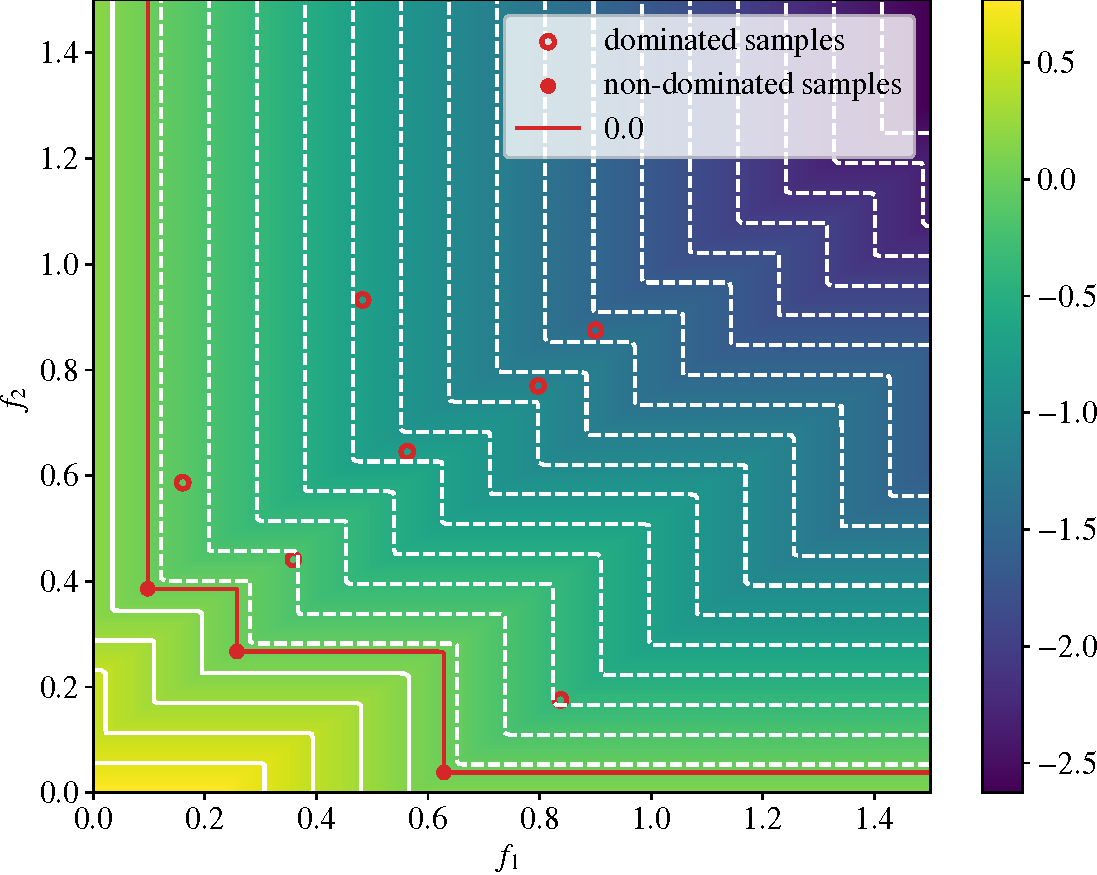
\includegraphics[width=\columnwidth]{figures/_objective_space_SAF_mu.pdf}
\end{subfigure}
\begin{subfigure}[t]{0.5\columnwidth}
    \includegraphics[width=\columnwidth]{figures/_objective_space_SMS.pdf}
\end{subfigure}
\caption{Visualised \safmu in two-objective space.}
\label{fig: saf_obj_space}
\end{figure}



We propose combining several components discussed in section \ref{section:related_work}, which have independently demonstrated advantages in efficient optimisation, be it in the domain of single or multi-objective optimisaiont. We propose a Bayesian approach to optimisation using GPs to model the objective function, and using the inexpensive and dominance preserving maximin function described in \cite{svenson2016multiobjective}, but forgoing the popular EI computation in favour of a more exploitative approach as explored in \cite{death2019greed}. To achieve this we will use the surrogate assisted EMO strategy with GP surrogates, as proposed by Emmerich \cite{emmerich2006single} using a multi-surrogate GP model, but using only the mean prediction of the surrogates when making predictions about new parameters, in order to emphasise exploitation, and hope that the complexity of MOPs will produce sufficient fortuitous exploration, without the need to actively pursue it. We propose combining the surrogate predictions of such maximia through an acquisition function which uses the maximin distance from the non-dominated observations. Pseudo-code for our proposed algorithm can be seen in Algorithm \ref{alg:ourAlg_pseudocde}.

\begin{algorithm}[t!]
  \SetAlgoLined
  \KwResult{minimiser of $\bff(\mathbf{x})$}
  \SetKwInOut{Input}{Input}
  \SetKwInOut{Output}{output}
  \SetKwComment{tcc}{}{}
  \SetCommentSty{textit}
  \DontPrintSemicolon
  \Input{$M$ - number of initial evaluations}
  \Input{$B$ - evaluation budget}
  \BlankLine
  %\textbf{Initialization}
  %\tcc*[l]{\textbf{Initialisation:}\hfill Generate initial samples}
  $X \gets \text{LatinHypercubeSampling}(\Omega, M)$ \label{alg: DSAF_LHS}
  \algremark{Generate initial samples}
  \For {$t = 1 \xrightarrow{} M$ \do}{ \label{alg:initial-start_DSAF}
    $\bff_t \gets \bff(\bx_t)$ \algremark{Expensively evaluate initial samples}
  } \label{alg:initial-end_DSAF}
  $\data  \gets \{(\bx_t, \bff_t)\}_{t=1}^M$
  \BlankLine
  
 \For{$t = M\xrightarrow{}B$ \do}{
 \For{$j=1\xrightarrow{}D$ \do}{
    $\theta_j \gets \text{train} \;\mathcal{GP}(\data)$\algremark{Train a GP for each objective}
    }
    $\mathcal{P} \gets \data$ \algremark{Select non-dominated evaluations according to \eqref{eqn: Pareto_set}}
    $\bx' \gets \underset{\mathbf{x}\in \Omega}{\argmax} \:
    \msaf(\mathbf{x}, \mathcal{P}, \theta_{1:D})$ \label{alg:opt-alpha_DSAF} \algremark{Find $\bx$ which maximises $\msaf$}
    $ \bff' \gets \bff(\bx')$ \label{alg:expensive_DSAF} \algremark{Expensively evaluate $\bx'$}
    $\data  \gets \data \cup \{(\bx', \bff' )\}$\algremark{Augment data}
 }
 $\mathcal{P} \gets \data$ \algremark{Select non-dominated evaluations according to \eqref{eqn: Pareto_set}}
 \Return $\mathcal{P}$ \algremark{Approximation to the Pareto set}
 \caption{SAF} 
 \label{alg:ourAlg_pseudocde} 
\end{algorithm}



\subsection{Related work}\label{section:related_work}
Bayesian approaches to solving EMOPs tend to use Gaussian Process surrogates and largely differ in the acquisition functions by which they select the parameters at which to next evaluate the true objective function.

The Acquisition functions which have proven most effective leverage measurement of the expected improvement to the $\mathcal{S}$-metric  \cite{emmerich2008computation}. That is the expected improvement to the hypervolume of objective space which is dominated by the the set of Pareto optimal solutions resulting from the inclusion of the GP model posterior prediction. First suggested by Emmerich \cite{emmerich2006single} as a pre-screening method for assisting GA optimisation, this approach naturally converges towards a set of solutions which well represent the Pareto front, as maximising the dominated hypervolume and finding the true Pareto set are equivalent \cite{fleischer2003measure}. 

However, the computation required for the dominated hypervolume scales poorly with both increased dimensionality of the objective space and increased number of Pareto-optimal solutions in the set of points evaluated by the true objective function. With even the most efficient algorithms scaling as $O(n^D)$, where $n$ is the number of points in the non-dominated set $\mathcal{P}\in\{\bx_1, \cdots, \bx_n\}$, for up to tri-objective problems, and potentially worse beyond that \cite{hupkens2014faster}. Furthermore increasing $D$ is often tied to a further increase in $n$ as there is greater likelihood of unique optimality in at least one combination of objectives and current methods of hypervolume computation quickly become intractable as the number of objectives increase. Nevertheless acquisition functions which compute the hypervolume improvement currently make up the stat-of-the art for EMO. SMS-EGO \cite{ponweiser2008multiobjective,wagner2010expected} performs well for problems with few objectives, and reduces the need for computation of the expected improvement to the hypervolume by applying a cheaper penalty function for predictions which fall within the region dominated $\mathcal{P}$. However, optimisation depends on the stetting of a well-placed reference point for the $\mathcal{S}$-metric calculation. Positioning of this reference vector requires some knowledge of the scales of the objective space, and poor positioning can bias the optimisation in favour of some objectives. 

Less expensive methods exist and involve dynamically altering the weighting applied to each objective during the optimisation process. Parego\cite{knowles2006parego}, does this by periodically generating a random weight vector which dictates the relative importance of each objective. Operating on a mono-surrogate model this is computationally efficient, and is well regarded in that respect, and while it will produce a set of solutions approximating the Pareto set, it converges in many more evaluations of the true objective function than SMS-EGO.

Alternatively, simpler methods which model the desirability of posterior predictions by interpolating the unexplored regions between observations in objective-space have been implemented with success. Keane \cite{keane2006statistical} uses the signed objective-space euclidean distance to the nearest point in $\mathcal{P}$ to interpolate between observations and then the EI is computed over this to form the acquisition function. However, as discussed in \cite{wagner2010expected} this fails to preserve the dominance relation, and is outperformed by SMS-EGO. Svenson \cite{svenson2016multiobjective} retains the dominance relation by using the maximin distance between the GP posterior prediction and the nearest point in the non-dominated set $\mathcal{P}$. The EI is then approximated using inexpensive Monte-Carlo estimation. In experiments on the DTLZ problems it is shown to perform comparably with measures of improvement to the dominated hypervolume. Although neither of these interpolation methods require setting of a reference point as in SMS-EGO, they are susceptible to bias depending on the scales of the objectives. Rahat \etal \cite{rahat2017alternative} compare a range of acquisition functions arguing that, although performance seems problem dependant, their proposed inexpensive minimum probability of improvement (MPoI) acquisition function performs comparably to using the hypervolume improvement, and similarly to the well known ParEgo algorithm \cite{knowles2006parego}, all such inexpensive acquisition functions however are surpassed consistently by the SMS-EGO state of the art.

In single-objective Bayesian optimisation, it has recently been suggested that exploitative optimisation methods are preferable over those which balance exploit/explore, such as EI, in problems where the complexity of the problem, causes low fidelity between the surrogate models and the objective function \cite{death2019greed}. They argue that exploitative methods are sufficiently \textit{fortuitously} exploitative in their nature without the need for active exploration. This work showed that deploying an exploitative, $\epsilon$-greedy' optimisation strategy was often preferable in problems where the parameter space was high-dimensional and thus the objective function complex.


\section{Experimental evaluation}
\subsection{Process}
In this section an analysis is conducted of the performance of \safmu over 150 evaluations of a set of challenging, synthetic MOPS. For comparison we also benchmark the performance against the state-of-the art \smsego \citep{ponweiser2008multiobjective} and the computationally efficient \parego \citep{knowles2006parego} and \mpoi as the infill criteria method suggested by Rahat \etal \citep{rahat2017alternative}. For \smsego we include the later improvements to the treatment of the objective space dominated by the attainment surface described by Wagner \etal \citep{wagner2010expected}, and the prior knowledge of the objective space required to set the reference point for the hypervolume calculation is assumed to be unknown. Instead the reference point is updated at each evaluation to the maximum value observed in each objective by the points in the current attainment surface multiplied by a factor of $1.5$. $\mref \gets \max(\pattainment)$. In order to test the second part of our hypothesis, that more explitative search will be beneficial, we also include the \EI based \minimax model proposed by Svenson \citep{svenson2016multiobjective}, (hereby denoted as \safei), and also a version of \smsego, where the uncertainty from the \GP is ignored, instead using mean prediction only, with no correction for $\epsilon$ (denoted \smsegomu.  

Each optimisation is started from 10 initial \lhs samples, over 31 repeat optimisations of each problem. The repeats are structured so that the same random seed and \lhs samples are used for all optimisation methods within each repeat, and the surrogate used in each of the surrogate methods is an identical \GP applied to the data normalised at each step to have $\mu=0$, $\sigma=1$. Where required the dominated hypevolume is calculated using the Fonseca hypervolume method \citep{fonseca2006improved}.

% \begin{itemize}
    % \item HOW CONDUCTED
    % \item analysis of performance on complex set of problems
    % \item to test two parts of hypothesis we test both mu and ei for saf and sms. And we compare to state of the art, efficient (Parego) and SOA SMS ego. AS well as MPOI method which has been shown to outperform other cheap infills (true?) 
    % \item over budget of 250 evaluations
    % \item 31 repeats of each optimiser
    % \item starting from 10 LHS samples
    % \item paired evaluations
    % \item where required hypervolumes calculated using Fonseca,
    % \item reference points selected from the maximum observed attainment front*1.5
    % \item GPs fitted to data scaled to std 1, mean 0. 
% \end{itemize}

The chosen objective functions on which to benchmark the different strategies are a subset the Walking Fish Group problems \citep{huband2005scalable} WFG1-WFG6, designed to build on the well-known DTLZ problem set \citep{deb2005scalable} by including deceptive functions and functions where the parameters dictating distance from, and position along the Pareto front are not separable. The dimensionality of the parameter-space $d$ for the WFG problems is scalable, as are the number of objectives $M$. We tested each function over three copnfigurations of each problem in WFG1-WFG6, with 2, 3 and 4 objectives, and parameter spaces ranging from 6-12 dimensions. The exception to this is WFG2, which was poorly optimised by all optimiser, and so had the parameter space reduced to the minimum permissable $d=[3, 4, 5]$ to aid convergence. A full table of the test functions can be seen in Table \ref{tab: f_table}.


\begin{table}[t]
    \setlength{\tabcolsep}{2pt}
    \sisetup{table-format=1.2e-1,table-number-alignment=center}
    \resizebox{0.5\textwidth}{!}{%
        \begin{tabular}{|l|r|l|r|l|}
            \hline
            Function &  $M$ & Domain & $d$ & Comment\\
            \hline
            WFG1 & 2, 3, 4 & $[0, 2d]^d$ & $3, 4, 5$ &  separable, uni-modal \\
            WFG2 & 2, 3, 4 & $[0, 2d]^d$ & $6, 6, 10$ & non-separable, multi-modal\footnotemark{}, discontinuous Pareto front \\
            WFG3 & 2, 3, 4 & $[0, 2d]^d$ & $6, 10, 10$ &  non-separable, uni-modal \\
            WFG4 & 2, 3, 4 & $[0, 2d]^d$ & $6, 8, 8$ & separable, multi-modal\\
            WFG5 & 2, 3, 4 & $[0, 2d]^d$ & $6, 8, 10$ & separable, deceptive\\
            WFG6 & 2, 3, 4 & $[0, 2d]^d$ & $10, 6, 12$ & non-separable, uni-modal\\
            \hline
        \end{tabular}}
        \caption{Objective functions to be assessed}\label{tab: f_table}
\end{table}
\footnotetext{multi-modal in only the first objective, uni-modal in $M>1$}

Two metrics are used to quantify the performance of each optimiser. The first is the dominated hypervolume (or $\mathcal{S}$-metric). This is a commonly used means of measuring convergence toward the Pareto front, but as it is also the driving force behind \smsego. As such we also compare measuremnets of the Inverted Generational Distance plus (\igd) \citep{ishibuchi2015modified}, calculated as:
\begin{equation}
    \migd(\pigdref, \pattainment) = \frac{1}{\abs{\pattainment}}\Bigg(
    \sum_{j=1}^{\abs{\pattainment}} d^{+}(\mathbf{z}_j, \mathbf{a})^{p}
    \Bigg)^{\frac{1}{p}}
\end{equation}
where $d_j$ is the nearest modified Euclidean distance drom $\mathbf{z}_j \in \pattainment$ to $\pigdref$, and $d^{+}$ is given by:
\begin{equation}
    d^+(\mathbf{z}, \mathbf{a}) = \sqrt{(\max\{a_1-z_1, 0\}+\cdots+\max\{a_m-z_m, 0\})}
\end{equation}
Measurements using \igd rely on a set of reference points $\pigdref$ on the problem's Pareto surface. In order to ensure no bias toward solutions found in localised regions of this surface it is important that the points be distributed evenly, which is not guaranteed once random samples have been mapped to the Pareto surface with the \textit{Shape Functions} described in the WFG function definitions. In order to achieve an even distribution, this we first sample an uneven, but dense population of points on this Pareto surface, and then calculate a set of evenly distributed points on the attainment surface generated using the methods described by Smith \etal \citep{smith2004dominance}. Attainment surface points which do not lie on the Pareto surface, were then discarded if their nearest neighbour in the set of Pareto optimal points, was greater than a certain threshold. This sampling method was used for all functions with the exception of WFG3, for which the Pareto surface is trivial to compute and sample evenly, and the reference points for the ellipsoidal WFG4 are shown in Figure \ref{fig: refpoints_wfg4}.  

\begin{figure}[t]
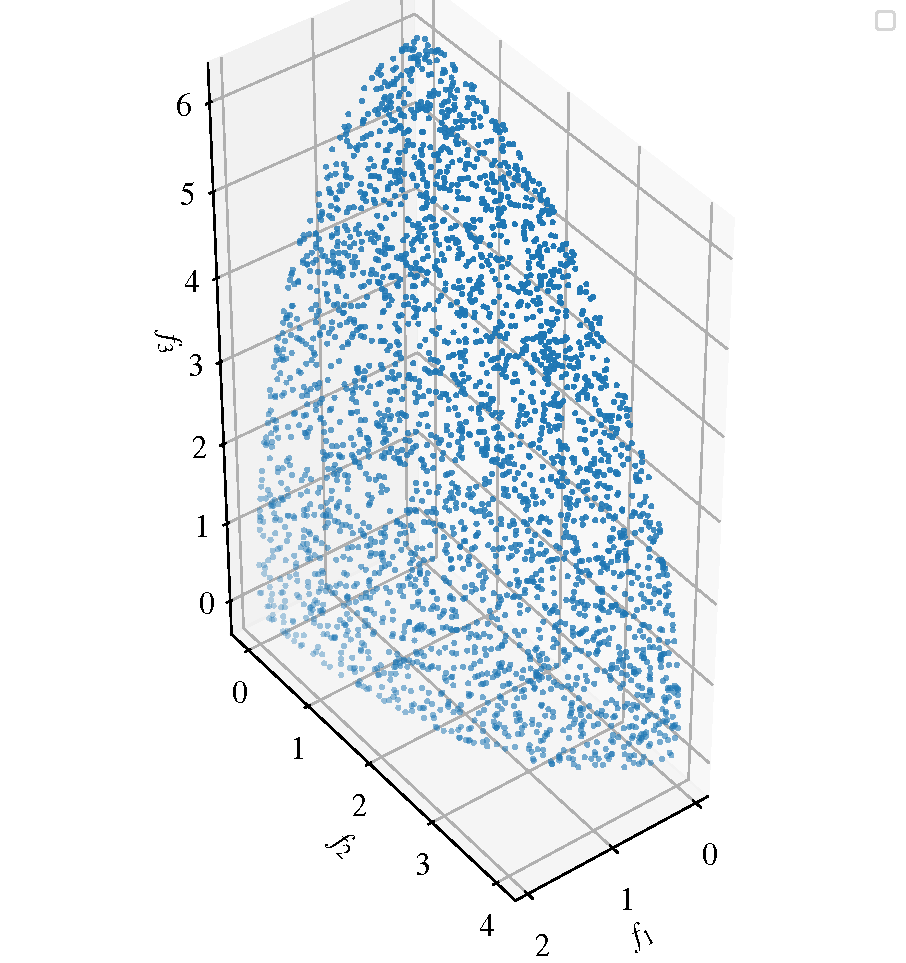
\includegraphics[width=\columnwidth]{figures/_IGD_refpoint_example_WFG4.pdf}
\caption{\igd reference points, for 3 objective WFG4.}
\label{fig: refpoints_wfg4}
\end{figure}

% \begin{itemize}
    % \item HOW ASSESSED
    % \item which problems chosen?
    % \item why problems chosen? build on DTLZ, include various features (multimodal, convex, separable). 
    % \item why d6? reduced dimensionality for wfg1 to facilitate finding better solutions
    % \item measurements taken using dominated hypervolume and igd+
    % \item igd+ samples taken by oversampling the pareto front, and then drawing a random sample from this using the attainment sampling techinique described in richards paper. 
    % \item results compared by their median value, with statistical equivlance tested using Holm-bonferoni corrected wilcoxen signed rank test. 
    % \item problem table
% \end{itemize}

\subsection{Discussion}
The results of the optimisations, as measured by \igd are summarised in table \ref{tab: igd_results}. The performances of the optimiser's are, as we may expect, somewhat problem dependant. After the full 150 budgeted evaluations of the objective functions, \safmu either had the lowest median \igd score, or did not differ significantly from the optimiser with the best score in 9 of the 18 tested problems, this is one more than the state-of-the art \smsego, but is equalled by the exploitative adaption \smsegomu. As we might expect, when measured by the $\mathcal{S}$-metric measure which the results are somewhat more favourable to \smsego and \smsegomu, with \safmu only being equivalent to the best performer on 9 optimisations, as opposed to \smsegomu's 9. 

Table \ref{tab: igd_results}  however, only considers a slice of the optimisation process, when the algorithms have largely converged. Figure \ref{fig: ranked_plots} shows average ranking of each optimiser across all repeats and all problems in the experimental setup, at each step of the optimisation process. Where neighbouring the difference between optimisations of similar rank have not been statistically significant, as judged by the Wilcoxon signed rank test, the two were assigned the same rank, hence the divergence as the optimisations progress. From this it is clear that \smsegomu performs best in the later stages, whether measuring by \igd or dominated hypervolume, but \safmu is second best by both of these measurement, although performance is similar to \smsego. 

It should be noted that all optimiser performed poorly on WFG2, with the majority of the Pareto Front left unexplored. \parego performed relatively well compared to the other functions, but many of the surrogate models were beaten by the \lhs benchmark here. It is worth noting that WFG2 is the only problem here with a discontinuous Pareto front, and in addition the manifold on which the Pareto front lies, extends into the hypervolume dominated by the Pareto front, meaning much of the dominated objective space is unattainable at each step, which is a feature unique to this function from those tested here but could be a factor in the poorer performance by optimisers which attempt to infill this space.


% \begin{itemize}
%     \item OVERALL
%     % \item As expected performance was problem-specific
%     % \item over the full 150 evaluations SAF-MU was the best performer or equivalent on 7 problems. The same as Sms EI. SMS-Mu was best with 9.
%     % \item For IGD+, saf-mu best on 9. SMS EI best on 8. SMS-MU also best on 9.
%     % % \item this only considers a snapshot of the optimisation process when the optimiser have largely converged. The ranked order can be seen in fig X. "ranks adjusted for equivalence". 
%     % \item WFG1 and 2 converged poorly by infill criteria methods
%     % \item WFG2 converged poorly by all methods
% \end{itemize}

\begin{table}[h]
\begin{subtable}[b]{\columnwidth}
\setlength{\tabcolsep}{2pt}
\sisetup{table-format=1.2e-1,table-number-alignment=center}
\resizebox{\columnwidth}{!}{%
\import{tables/}{igd_table_1.tex}}
\end{subtable}
\begin{subtable}[b]{\columnwidth}
\setlength{\tabcolsep}{2pt}
\sisetup{table-format=1.2e-1,table-number-alignment=center}
\resizebox{\columnwidth}{!}{%
\import{tables/}{igd_table_2.tex}}
\end{subtable}
\begin{subtable}[b]{\columnwidth}
\setlength{\tabcolsep}{2pt}
\sisetup{table-format=1.2e-1,table-number-alignment=center}
\resizebox{\columnwidth}{!}{%
\import{tables/}{igd_table_3.tex}}
\end{subtable}
\caption{\igd results after 150 function evaluations.}
\label{tab: igd_results}
\end{table}

The hypothesis that search based on the mean prediction could offer improvements over EI approaches appears to be borne out by the results. \smsegomu performs similarly well to \smsego, with few exceptions. There certainly seems to be no advantage to incorporating the uncertainty from the model. This however is not a true EI method, and does not integrate the posterior prediction to get the expected improvement, but rather calculates the expected improvement to the dominated hypervolume based on the surrogate prediction. \safei is more similar to true EI, though it uses a Monte-Carlo integration to estimate the model EI. The performance of \safei is significantly worse than that of \safmu, never once outperforming the mean prediction version. This supports the ideas put forward by DeAth \citep{death2019greed}, that in problems which are complex to model the fortuitous exploration resulting from low surrogate fidelity is sufficient to explore the parameter space.

It appears that broadly speaking \safmu does not surpass the performance of \smsego significantly, but is as good in the majority of cases tested, though the nature of the  function being optimised remains a key factor in which optimiser performs best. 

\begin{figure}[t]
\begin{subfigure}[b]{\columnwidth}
         \centering
         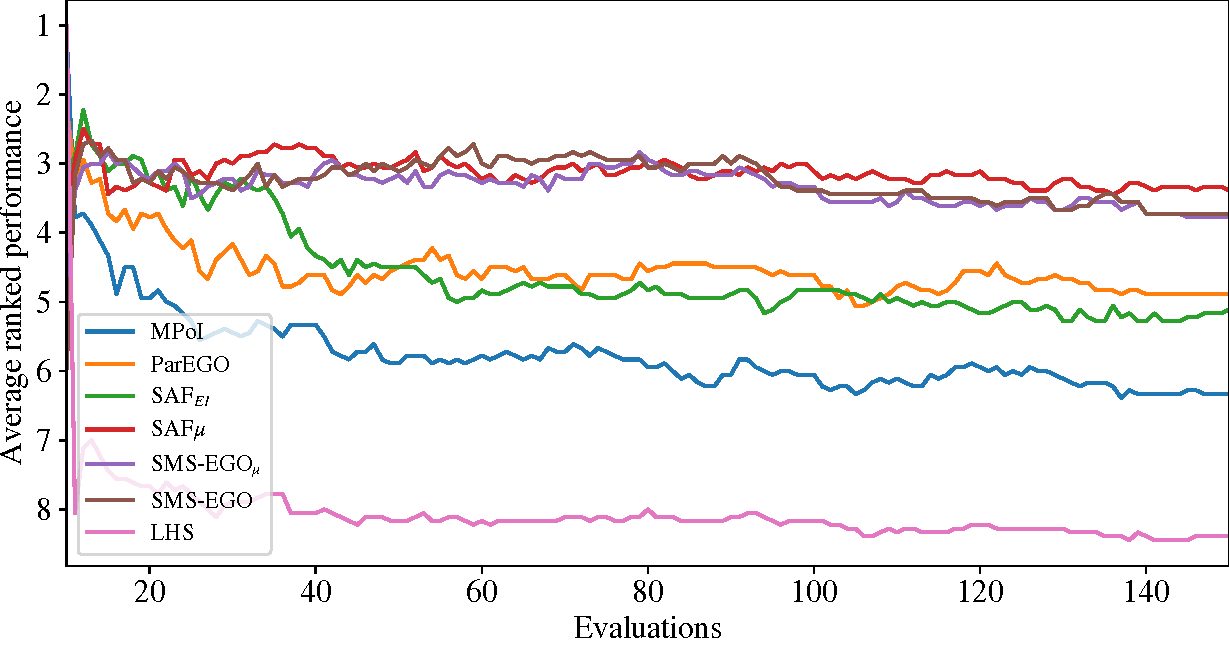
\includegraphics[width=\columnwidth]{figures/_ranked_performance_plot_hv.pdf}
        %  \caption{}
        %  \label{fig: ranked_hv_plot}
     \end{subfigure}
\begin{subfigure}[b]{\columnwidth}
         \centering
         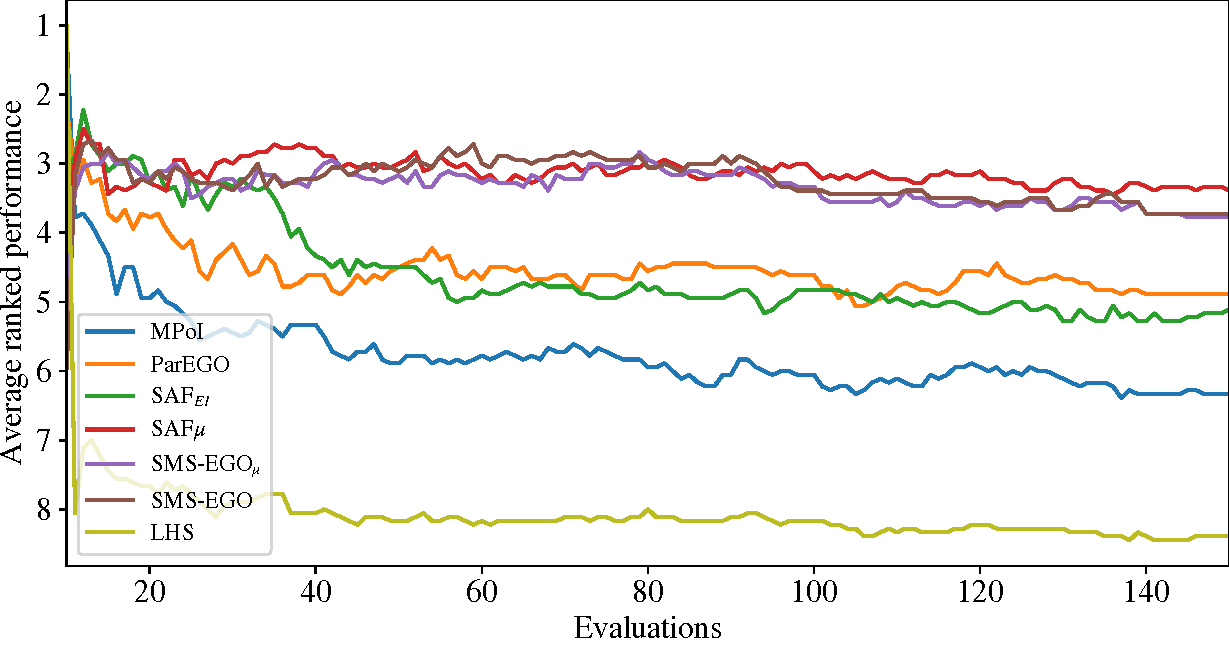
\includegraphics[width=\columnwidth]{figures/_ranked_performance_plot_igd.pdf}
        %  \caption{}
        %  \label{fig: ranked_igf_plot}
     \end{subfigure}
\caption{ranks}
\label{fig: ranked_plots}
\end{figure}

    

\begin{table}[t]
    \setlength{\tabcolsep}{2pt}
    \sisetup{table-format=1.2e-1,table-number-alignment=center}
    \resizebox{0.5\textwidth}{!}{%
    \begin{tabular}{|l|l|l|}
        \hline
        Optimiser name & surrogate  & Comment\\
        \hline
        Saf ei & Multi & EI version of SAF, as proposed in \cite{svenson2016multiobjective}. \\
        Saf $\mu$ & Multi & Our proposed Optimiser. (See Alg. \ref{alg:ourAlg_pseudocde}) \\
        SMS-EGO: ei & Multi & Current SOA \\
        SMS-EGO: $\mu$ & Multi & Modification to current SOA to be more exploitative.\\
        ParEgo & Mono & Efficient computation \\
        MPoI & Multi & Benchmark for EMO over infill criteria approach. \\
        LHS & None & Baseline comparison to pseudo-uniform sampling of parameter space. \\
        \hline
    \end{tabular}}
    \caption{Optimisation strategies to be compared}\label{tab1}
    \label{table:alg_table}
\end{table}


The WFG problems are intentionally constructed to cover significantly different numerical ranges in the domains of each of their objectives. This presents a problem to the DHV measurement, as the computation of the HV depends onheavily on the scales of the objectives. A common solution to this is to optimise a scaled version of the WFG problems where the ranges of each dimension have been normalised, and to set the reference point for the DHV measurement within this scaled objective space, equidistant from the origin \cite{}. To do this is to assume prior knowledge about the objective function, information which is not typically available in real-world problems. SMS-EGO uses the dominated hypervolume measurement in its process of assessing candidate solutions, and to scale the objectives a priori and provide an ideally positioned reference point is not realistic in a real application. Furthermore setting the DHV reference point for SMS-EGO identically to that against which it is assessed will inevitably give SMS-EGO an unfair advantage, when assessed by the DHV criterion. Instead we will require SMS-EGO to set its own reference point and scale the objectives accordingly. This will be done dynamically during the optimisation in order to normalise the range of each objective present in the non-dominated set of observations. 



\subsection{Conclusion}
When optimising expensive, multi-objective problems efficient use of objective evaluations is critical to convergence within the constraining budget. Current state-of-the-art methods for optimising such problems in few evaluations rely on expensive hypervolume computation which can itself become prohibitively costly as the number of objectives is scaled, and the number of non-dominated solutions in the attainment surface increases. The state-of-the art method is benchmarked on a comprehensive set of synthetic test problems, and an optimisation method based on a cheap, exploitative, \minimax distance infill criteria method from the attainment surface is presented and shown to be similarly effective across the test problems.

By benchmarking on the same set of problems we further show that leveraging the expected improvement offer no improvement over mean prediction when it comes to complex EMO problems
\begin{enumerate}
    \item We have introduced SAF-mean as a means of solving EMOs.
    \item Showed SAF-mean similar to SmsEgo performance, without need for hypervolume itegration.
    \item We have further shown that EI based models are flawed , with high dimensional feature spaces and offered an explanation, with evidence, for why this is. 
    \item Further work: Not needing to leverage posterior prediction uncertainty opens the EMO strategy up to a wider range of surrogate models. Some of which (e.g. Random Forests) are not as severely limited by the \textit{curse of dimensionality} as GPs, and this could allow EMO to be applied to many objective problems. 
\end{enumerate}

\section{Definitions required}
\begin{enumerate}
    \item Objective space
    \item Domination
\end{enumerate}


\section{Consideratios/ammendments to be made}
\begin{itemize}
    \item hyphenate multisurrogate, monosurrogate, single surrogate
    \item check for consistency in parameters vs inputs, 
    \item Do i need to explain traingp in algorithms?
    \item MOOP vs MOP vs MOO<- pick one
    \item define HV
    \item state of the art vs state-of-the-art
    \item check meaning of S-metric
\end{itemize}

\begin{acks}
The authors acknowledge ...
\end{acks}





\bibliographystyle{ACM-Reference-Format}
\bibliography{bibliography}

\end{document}

%%% Local Variables:
%%% mode: latex
%%% TeX-master: t
%%% End:

